\documentclass[border=20pt,preview]{standalone}
\usepackage{tikz}
\usepackage{xcolor}
\usepackage{amsmath}
\usetikzlibrary{arrows}
\begin{document}

\begin{center}
    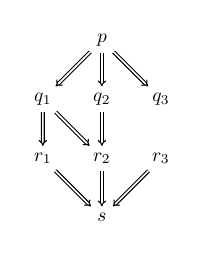
\begin{tikzpicture}[scale=1.5]
        \pgfmathsetmacro{\separate}{0.5}

        \node[scale=0.7] (p) at (0, 0) {\(p\)};

        \node[scale=0.7] (q1) at (-\separate, -\separate) {\(q_1\)};
        \node[scale=0.7] (q2) at (0, -\separate) {\(q_2\)};
        \node[scale=0.7] (q3) at (\separate, -\separate) {\(q_3\)};

        \node[scale=0.7] (r1) at (-\separate, -2 * \separate) {\(r_1\)};
        \node[scale=0.7] (r2) at (0, -2 * \separate) {\(r_2\)};
        \node[scale=0.7] (r3) at (\separate, -2 * \separate) {\(r_3\)};

        \node[scale=0.7] (s) at (0, -3 * \separate) {\(s\)};

        \draw[-implies, double] (p) -- (q1);
        \draw[-implies, double] (p) -- (q2);
        \draw[-implies, double] (p) -- (q3);

        \draw[-implies, double] (q1) -- (r1);
        \draw[-implies, double] (q1) -- (r2);
        \draw[-implies, double] (q2) -- (r2);

        \draw[-implies, double] (r1) -- (s);
        \draw[-implies, double] (r2) -- (s);
        \draw[-implies, double] (r3) -- (s);
    \end{tikzpicture}
\end{center}

\end{document}
